% Geometry, font
\documentclass[12pt, letter]{article}
\usepackage[margin=0.8in]{geometry}
\usepackage[T1]{fontenc}
\usepackage{fourier}
\usepackage{titling}
\setlength{\droptitle}{-5em} 
\usepackage[parfill]{parskip}
\usepackage{graphicx}

% Math stuff
\usepackage{amssymb}
\usepackage{amsmath}
\usepackage{bm}

\author{Zach Neveu}
\title{ Analysis, Big O and Growth of Functions }

\begin{document}
\maketitle

\section{Book Keeping}%
\label{sec:book_keeping}
\begin{itemize}
	\item Reading posted
	\item Lab 1 available
\end{itemize}

\section{Analysis of Algorithms}%
\label{sec:analysis_of_algorithms}
\begin{quote}
	Problem: a general description of input parameters and the properties that an optimal solution should have
\end{quote}
\begin{quote}
	Instance: a specific example of a problem with all parameters specified
\end{quote}
\begin{itemize}
	\item Example: Given a weighted graph, find the cheapest Hamiltonian Cycle (TSP)
	\item A "problem" can have many instances
\end{itemize}

\begin{figure}[h]
	\centering
	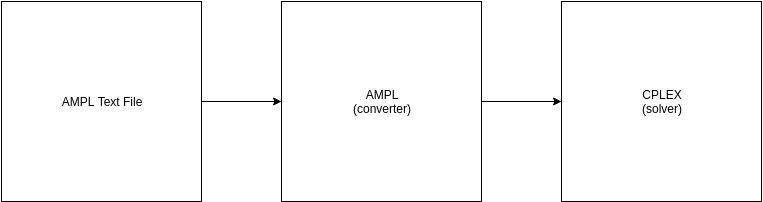
\includegraphics[width=0.5\textwidth]{Page-1}
	\caption{instance\_problem}
	\label{fig:instance_problem}
\end{figure}

\begin{itemize}
	\item An algorithm solves all instances of problem
	\item Many algorithms, what is most efficient?
	\item What is efficient?
	\begin{itemize}
		\item Memory
		\item Time
		\item CPU cycles
		\item Disk Space
		\item I/O bandwidth
		\item Power
	\end{itemize}
	\item Efficiency usually defined as using smallest time
	\item Index runtimes by instance size
	\item "Instance Size" not always well defined - can have multiple params (edges, nodes)
\end{itemize}

\section{Example: Insertion Sort}%
\label{sec:example_insertion_sort}

\begin{figure}[h]
	\centering
	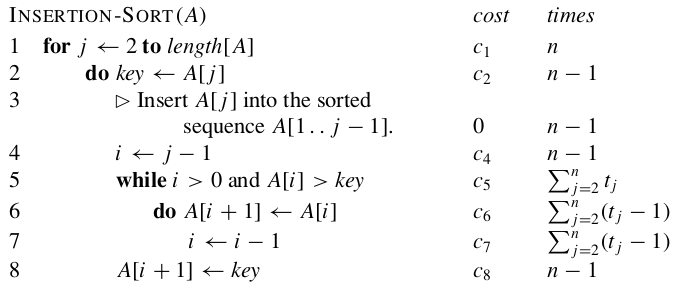
\includegraphics[width=0.8\textwidth]{imgs/insertion_sort.png}
	\caption{Cor p.24}
	\label{fig:imgs-insertion_sort-png}
\end{figure}
\begin{itemize}
	\item Best case: already sorted. $T(j)=1, T(n)=an+b \rightarrow$ linear
	\item Worst case: reverse sorted: $T(j)=j, T(n) = \frac{n(n+1)}{2} \approx an^2+bn+c\rightarrow$ quadratic
\end{itemize}

\begin{quote}
	Time Complexity Function: The largest amount of time for an algorithm needed to solve the problem for a given instance size.
\end{quote}

\begin{itemize}
	\item Even Time-Complexity function considered too complicated for daily use
	\item Asymptotic notation used instead
\end{itemize}

\section{Asymptotic Notation}%
\label{sec:asymptotic_notation}
For a given function $g(n)$, $O(g(n))=f(n)$ there exist positive constants $k$ and  $n_0$ such that  $f(n) \le Kg(n)$ for all  $n \ge n_0$ \\
Less formally: $O(g(n))$ is the set of functions that are asymptotically less than $g(n)$ for large  $n$.

\subsection*{Example}
I claim that $f(n) = an^2_bn+c = O(n^2) $. If so, then there should exist positive constants $k$ and  $n_0$ such that
\begin{gather*}
an^2+bn+c \le kn^2 \\
a+b/n +\frac{c}{n^2} \le k \\
k = a+1 \\
n_0\ is\ intersection
\end{gather*}

\subsection*{Summary}
\begin{itemize}
	\item For insertion sort, worst case runtime (time complexity function) is $an^2+bn+c$ so the complexity is $O(n^2)$ \\
	\item Also $O(n^{3}), O(n^{4})$ etc.
	\item Worst case runtime is $O(n^2)$
	\item Worst case runtime \textbf{itself} is upper bound on run time
	\item $O(n^2)$ is then an upper bound on the general runtime as well!
\end{itemize}

\begin{quote}
	Polynomial-time Algorithm: an algorithm whose time complexity function is $O(p(n))$ for some polynomial $p(n)$
\end{quote}

\begin{quote}
	Exponential-time Algorithm: an algorithm that is not polynomial time
\end{quote}

\subsection*{EXPONENTIAL VERY BAD}

\end{document}
